
\begin{figure}[ht]
  \begin{widepage}
    \centering
    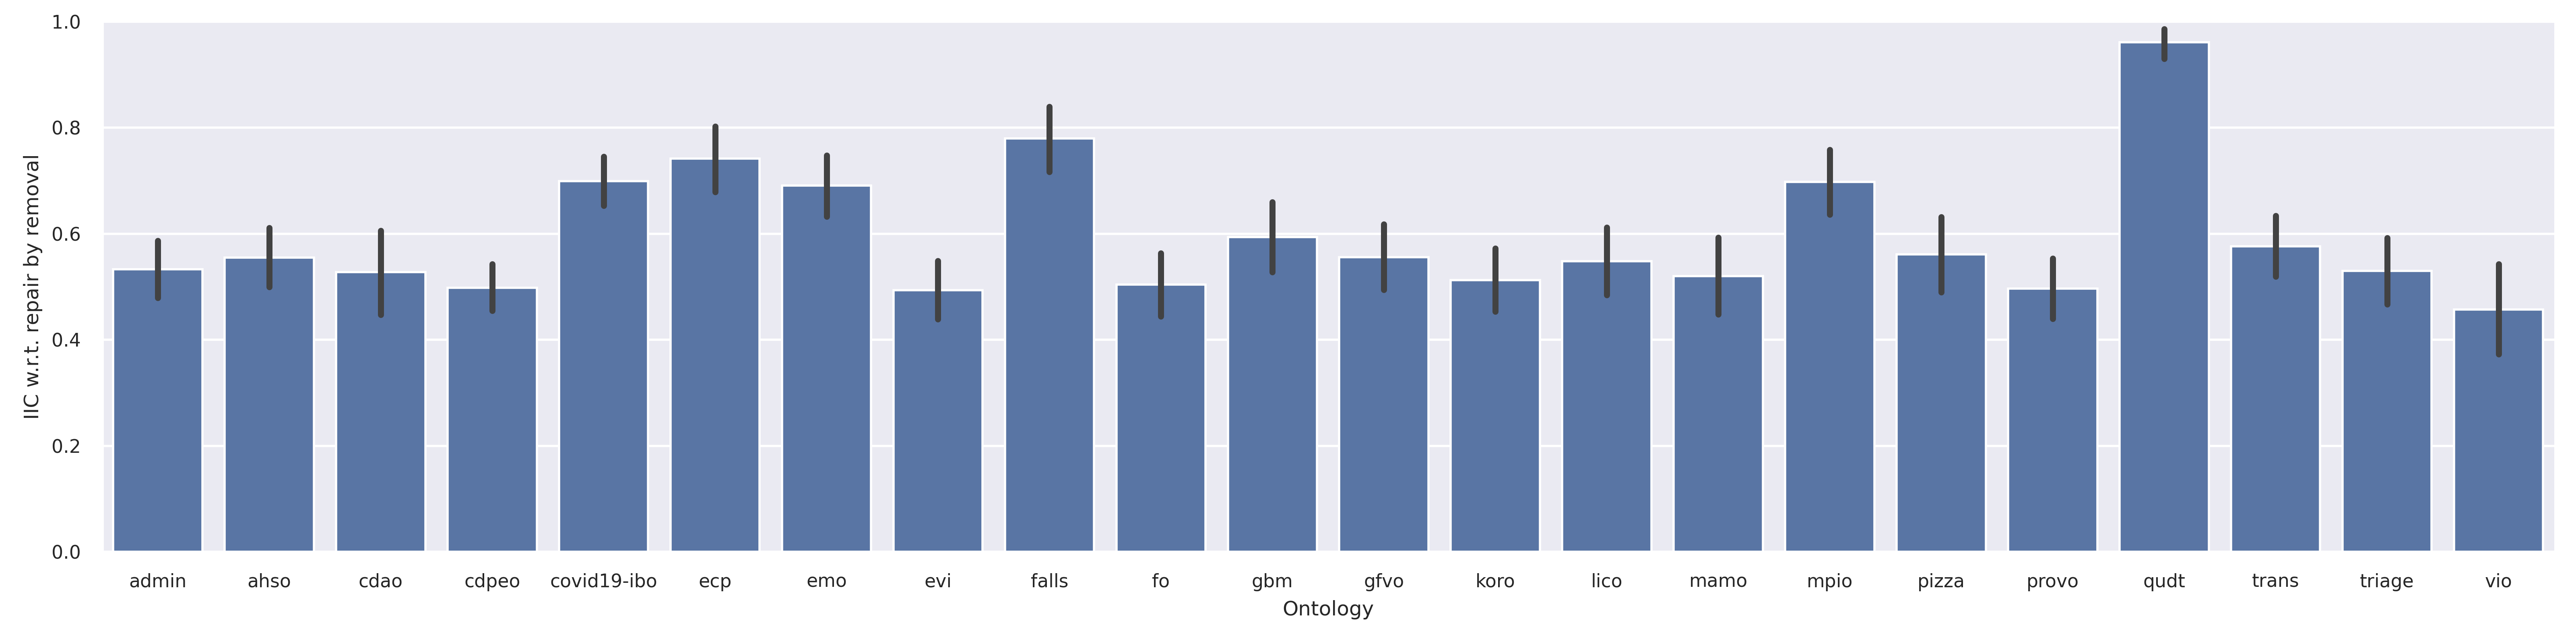
\includegraphics[width=\textwidth]{resources/iic-remove-ontology-bar.png}
  \end{widepage}
  \caption{Mean IIC with respect to repair via removal per ontology. The error bars show the 95\% confidence interval.}
\end{figure}

\begin{figure}[ht]
\begin{widepage}
  \centering
  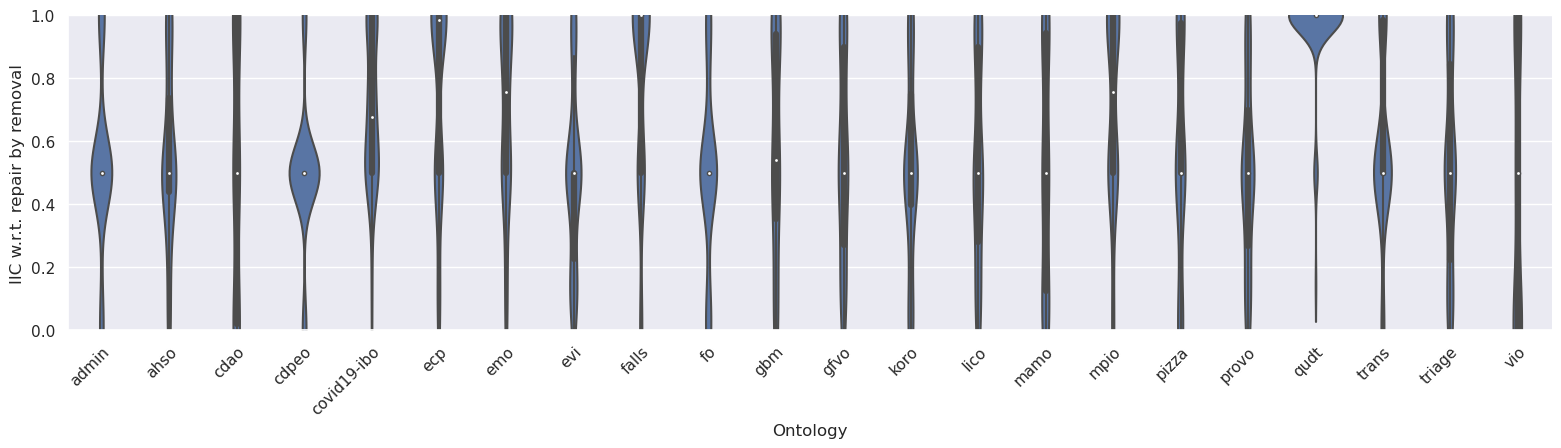
\includegraphics[width=\textwidth]{resources/iic-remove-ontology-violin.png}
\end{widepage}
\caption{Distribution of IIC with respect to repair via removal per ontology.}
\end{figure}

\begin{figure}[ht]
  \begin{widepage}
    \centering
    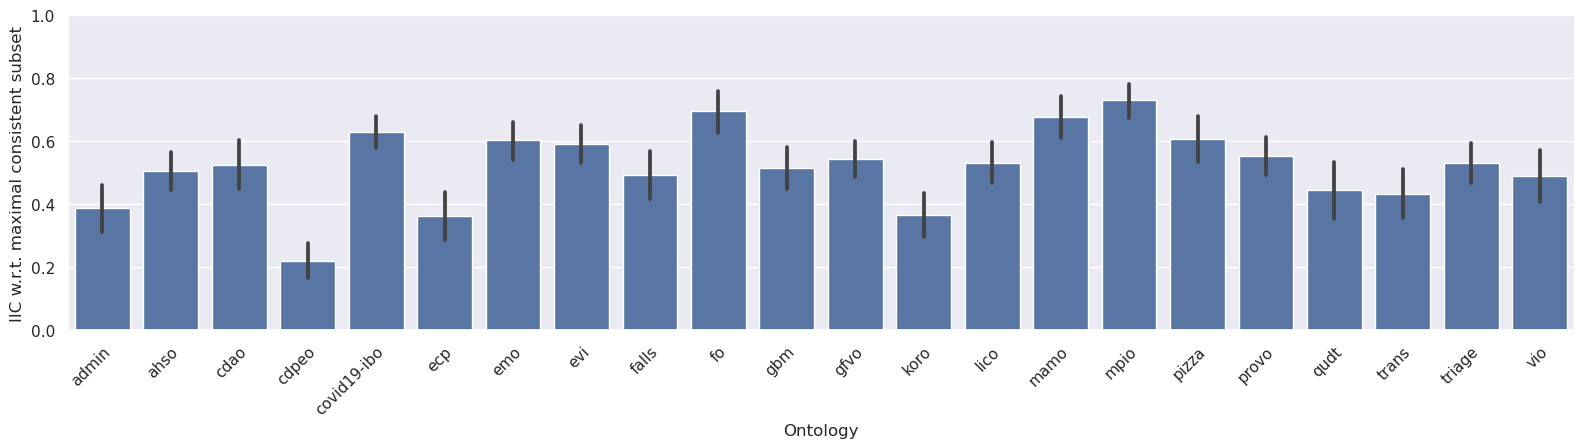
\includegraphics[width=\textwidth]{resources/iic-mcs-ontology-bar.png}
  \end{widepage}
  \caption{Mean IIC with respect to repair via a random maximal consistent subset per ontology. The error bars show the 95\% confidence interval.}
\end{figure}

\begin{figure}[ht]
    \begin{widepage}
      \centering
      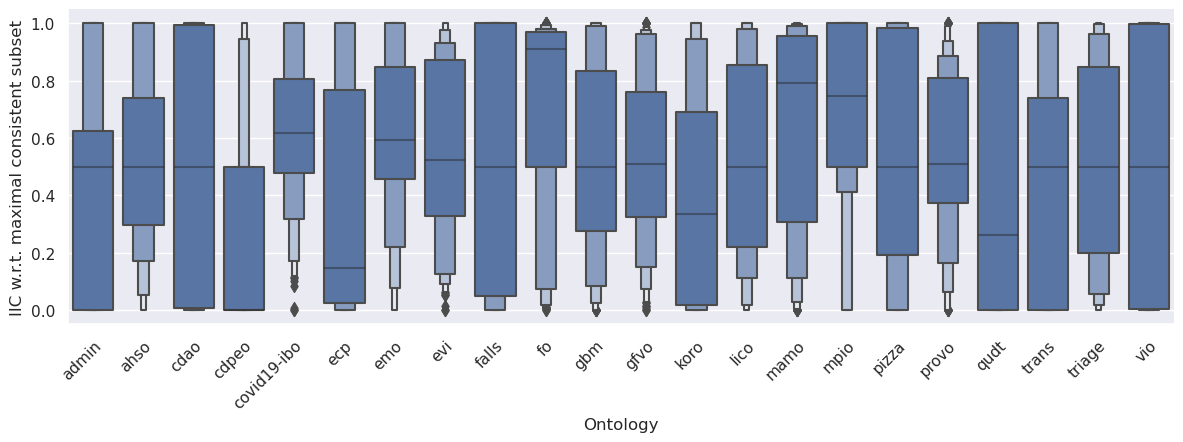
\includegraphics[width=\textwidth]{resources/iic-mcs-ontology-violin.png}
    \end{widepage}
    \caption{Distribution of IIC with respect to repair via a random maximal consistent per ontology.}
\end{figure}

\begin{figure}[ht]
  \begin{widepage}
    \centering
    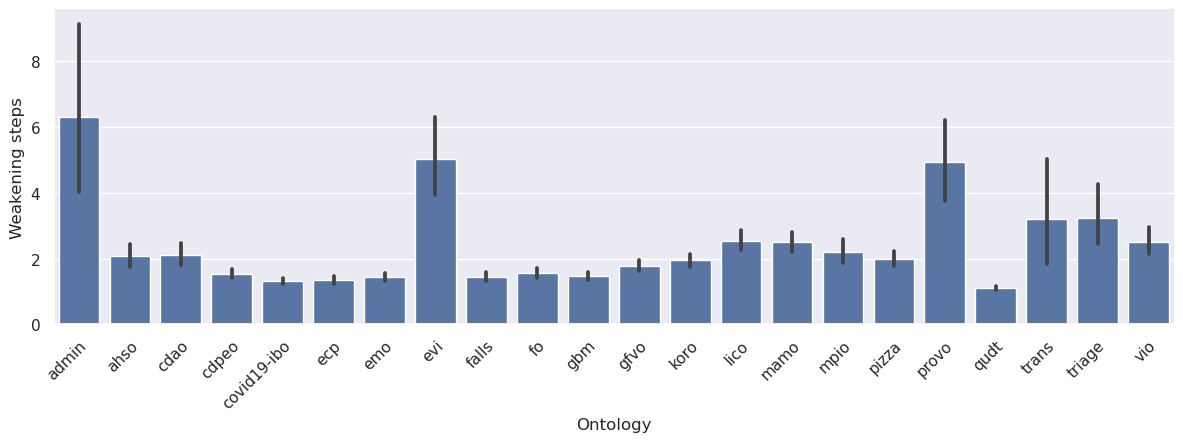
\includegraphics[width=\textwidth]{resources/steps-ontology-bar.png}
  \end{widepage}
  \caption{Mean number of weakening steps needed for repairing the ontology. The error bars show the 95\% confidence interval.}
\end{figure}

\begin{figure}[ht]
  \begin{widepage}
    \centering
    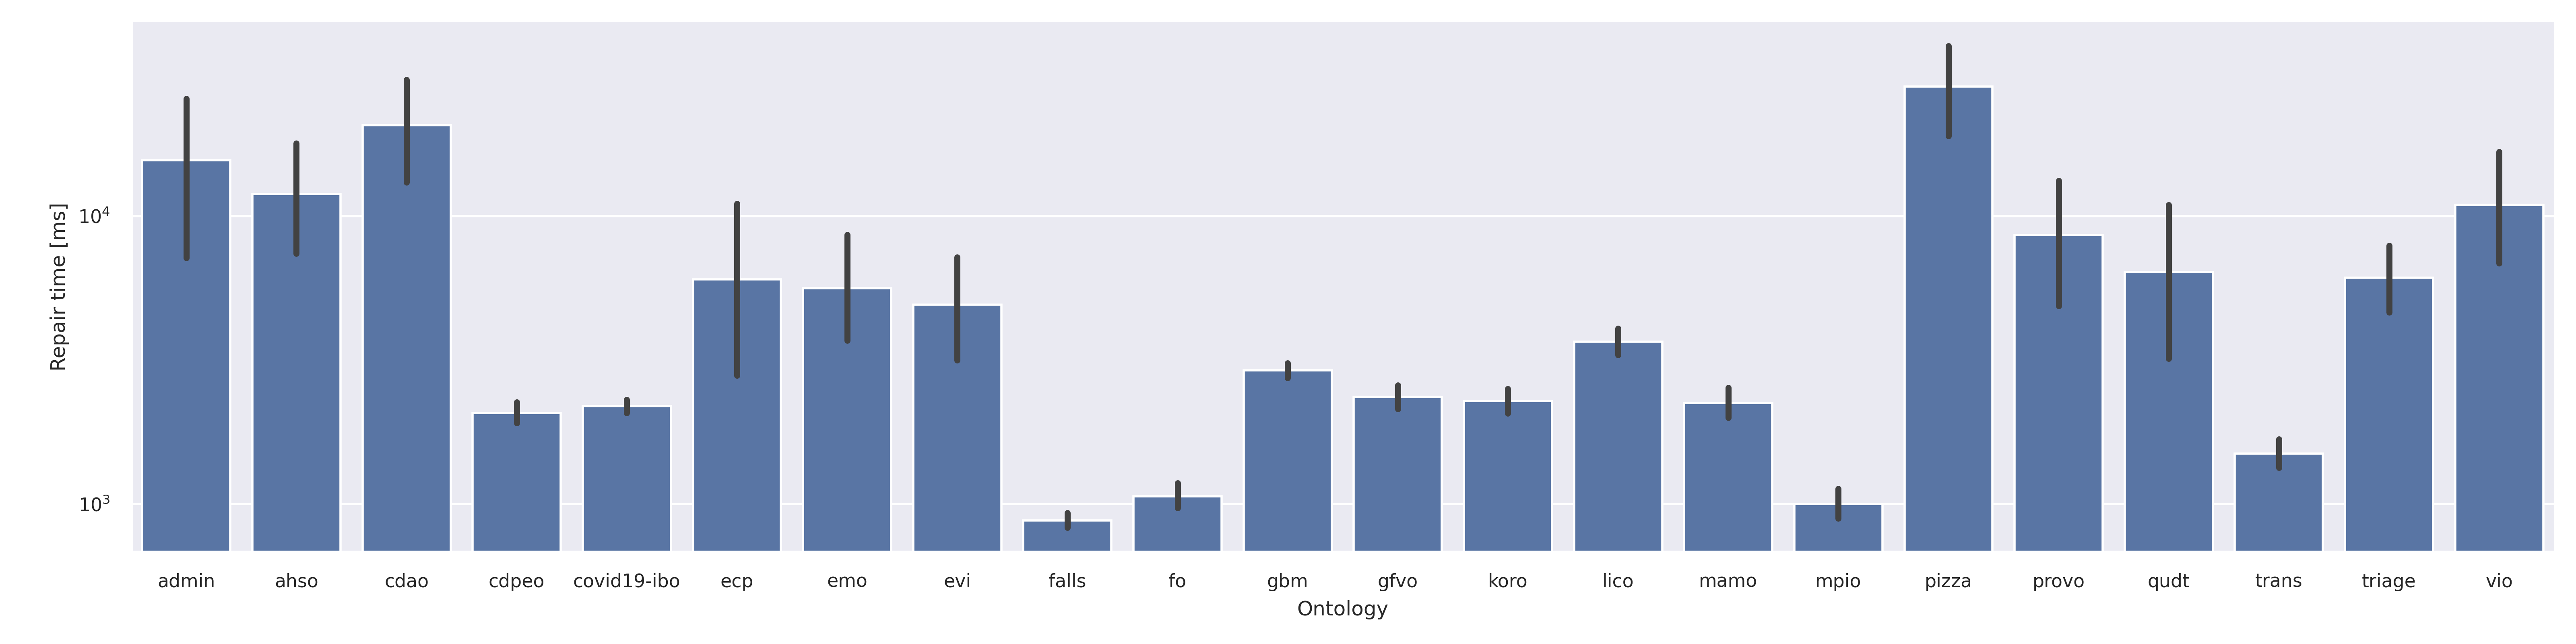
\includegraphics[width=\textwidth]{resources/time-ontology-bar.png}
  \end{widepage}
  \caption{Mean execution time required for repairing using axiom weakening by ontology. The error bars show the 95\% confidence interval. Attempts that failed by timeout were not considered.}
\end{figure}

\begin{figure}[ht]
    \begin{widepage}
      \centering
      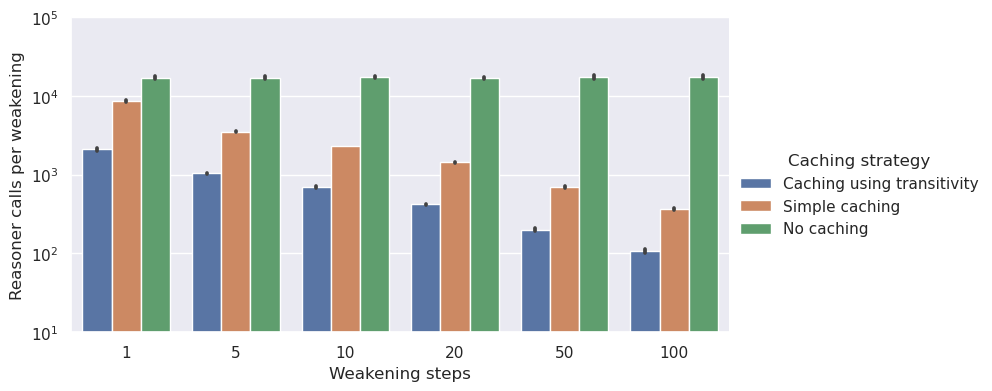
\includegraphics[width=\textwidth]{resources/calls-cache-bar.png}
    \end{widepage}
    \caption{Average reasoner calls with different caching strategies when executing axiom weakening of random axioms. Results are the average between the following ontologies: admin, cdpeo, emo, gbm, gfvo, koro, and mamo. Each consistency or entailment query made to the reasoner count as one call.}
\end{figure}

\begin{figure}[ht]
    \begin{widepage}
      \centering
      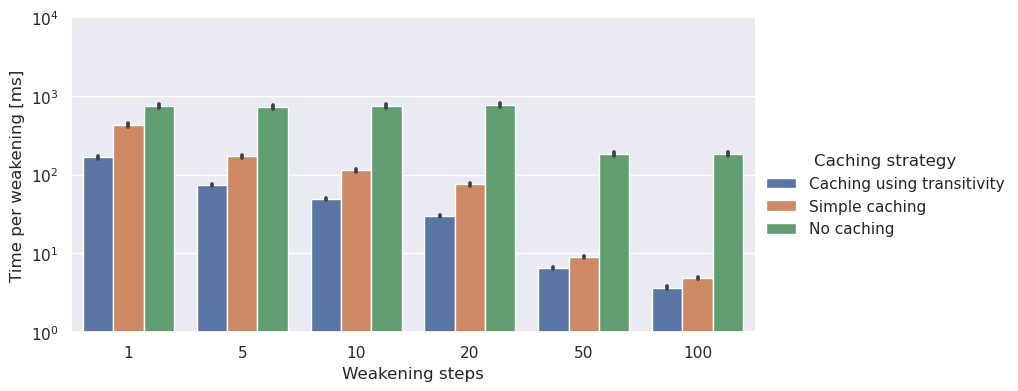
\includegraphics[width=\textwidth]{resources/time-cache-bar.png}
    \end{widepage}
    \caption{Average time required per application of the axiom weakening operator with different caching strategies when executing axiom weakening of random axioms. Results are the average between the following ontologies: admin, cdpeo, emo, gbm, gfvo, koro, and mamo. The results are averaged for the reasoners FaCT++, JFact, Openllet, and HermiT.}
\end{figure}

\begin{figure}[ht]
    \begin{widepage}
      \centering
      
\includegraphics[height=0.9\textheight]{resources/calls-cache-ontology-bar.png}
    \end{widepage}
    \caption{Average reasoner calls with different caching strategies when executing axiom weakening of random axioms per ontology. Each consistency or entailment query made to the reasoner count as one call.}
\end{figure}

\begin{figure}[ht]
    \begin{widepage}
      \centering
      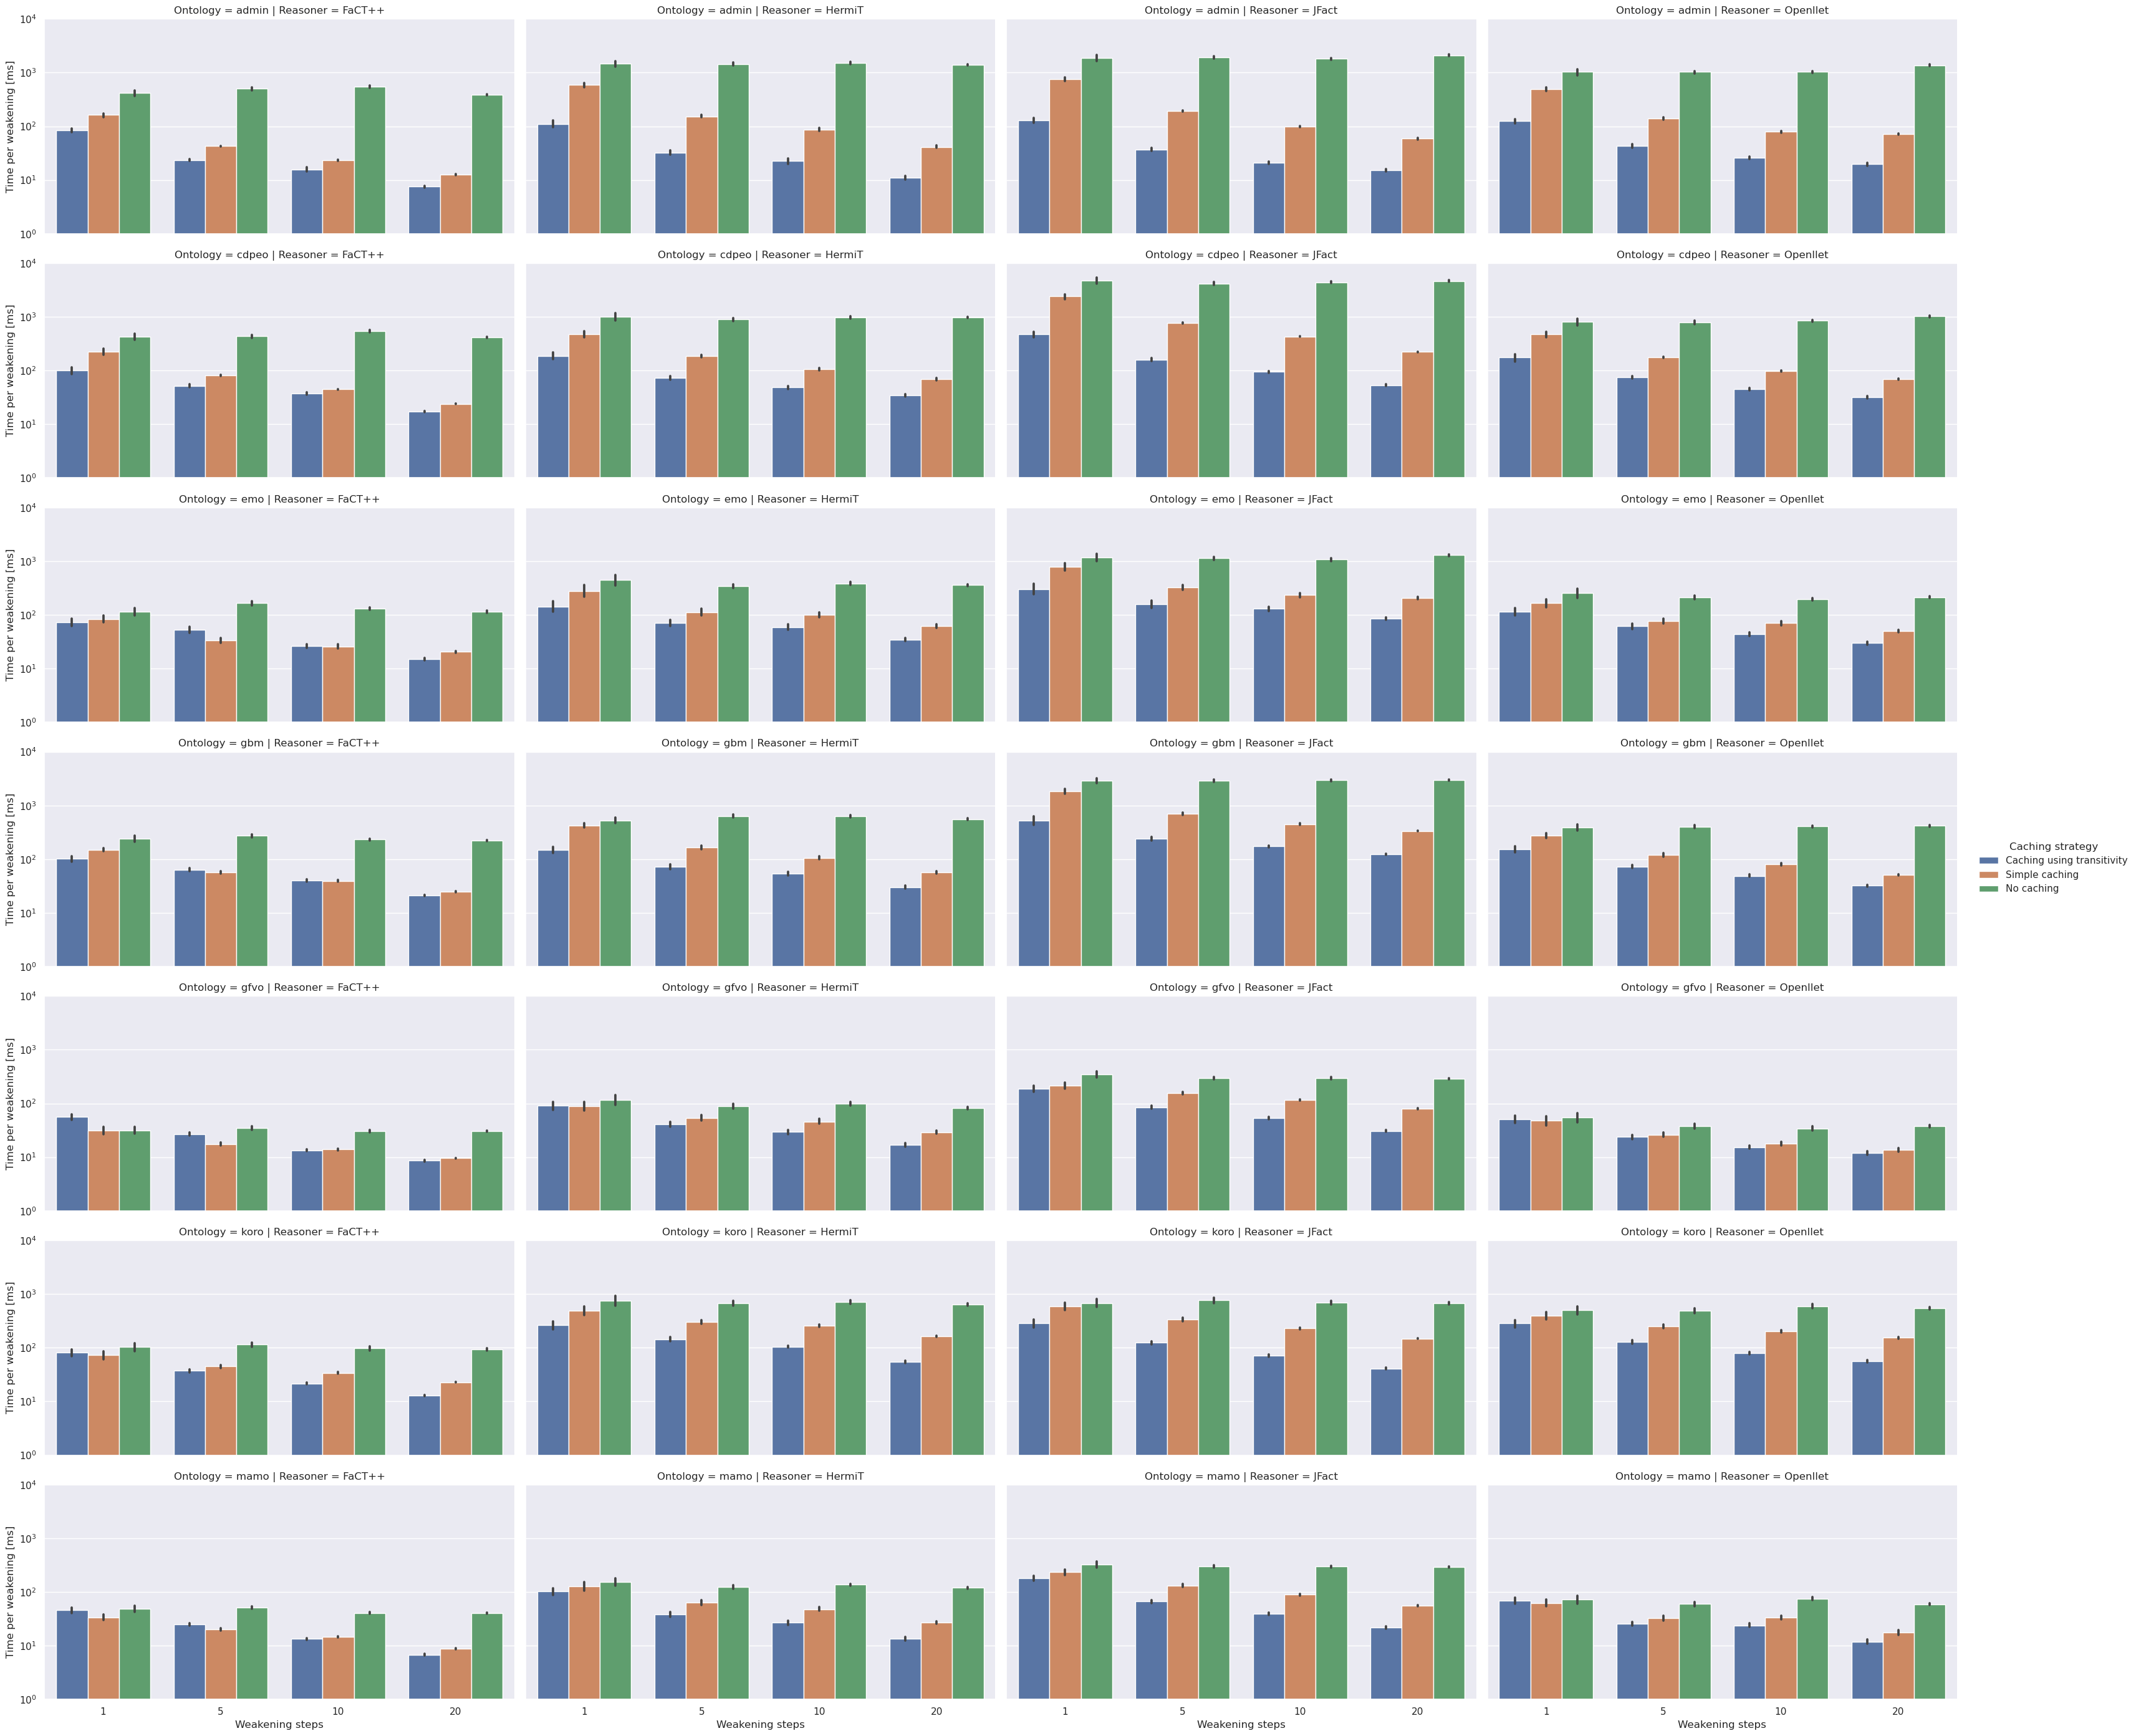
\includegraphics[width=\textwidth]{resources/time-cache-ontology-reasoner-bar.png}
    \end{widepage}
    \caption{Average time required per application of the axiom weakening operator with different caching strategies when executing axiom weakening of random axioms per ontology and reasoner.}
\end{figure}
